\documentclass[a4paper,12pt]{article}
\usepackage{graphicx}
\begin{document}
\title{\Large{\textbf{Securing our Social Lives From Networking Attacks}}}
\author{Himanshu Pandey, Ujjwal Khanduri\\ National Institute of Technology, Uttarakhand \\ Email: himanshup.csebt18@nituk.ac.in, ujjwalk.csebt18@nituk.ac.in}
\date{April 20,2021}

\maketitle

\section*{Abstract}

As the digital era matures, cyber security evolves and software vulnerabilities
diminish, people however, as individuals,
are more exposed today than ever before.
Presently, one of the most practiced and effective penetration attacks are social rather
than technical, so efficient in fact, that these
exploits play a crucial role to support the
greatest majority of cyber assaults. Social
Engineering is the art of exploiting the human flaws to achieve a malicious objective.
In the context of information security, practitioners breach defences to access sensitive
data preying particularly upon the human
tendency towards trust. Cyber criminals induce their victims to break security protocol forfeiting confidential information propitious for a more targeted attack. Disastrously, in many cases, targets are manipulated to involuntarily infect and sabotage
the system themselves.

\section{Introduction}

Social engineering is the term used for a broad range of malicious activities accomplished through human interactions. It uses psychological manipulation to trick users into making security mistakes or giving away sensitive information.

Social engineering attacks happen in one or more steps. A perpetrator first investigates the intended victim to gather necessary background information, such as potential points of entry and weak security protocols, needed to proceed with the attack. Then, the attacker moves to gain the victim’s trust and provide stimuli for subsequent actions that break security practices, such as revealing sensitive information or granting access to critical resources.
What makes social engineering especially dangerous is that it relies on human error, rather than vulnerabilities in software and operating systems. Mistakes made by legitimate users are much less predictable, making them harder to identify and thwart than a malware-based intrusion.

\section{Literature Survey}

Social engineering attacks may combine
the different aspects previously discussed,
namely: human, computer, technical, social, and physical-based. Examples of social engineering attacks include phishing,
impersonation on help desk calls, shoulder surfing, dumpster diving, stealing important documents, diversion theft, fake
software, baiting, quid pro quo, pretexting, tailgating, Pop-Up windows, Robocalls, ransomware, online social engineering, reverse social engineering, and phone
social engineering.
We shall always look forward to where the
system is weak and the attacker can get the
information.

\section{Types of attacks}

\subsection{Phishing}
Phishing is a cyber attack that uses disguised email as a weapon. The goal is to trick the email riciepent into believing that the message is something they want or need - a request from their bank, for instance, or a note from someone in their company - and to click a link or download an attachment. 

What really distinguishes phishing is the form the message takes: the attackers masquerade as a trusted entity of some kind, often a real or plausibly real person, or a company the victim might do business with. It's one of the oldest types of cyberattacks, dating back to the 1990s, and it's still one of the most widespread and pernicious, with phishing messages and techniques becoming increasingly sophisticated.

\subsubsection{Approach}
\\
We will use a tool named blackeye (https://github.com/An0nUD4Y/blackeye) to setup the frontend and backend of the phishing sites. \\
\\
\\
\\
\\
\\
\\
\\

\begin{figure}[htbp]
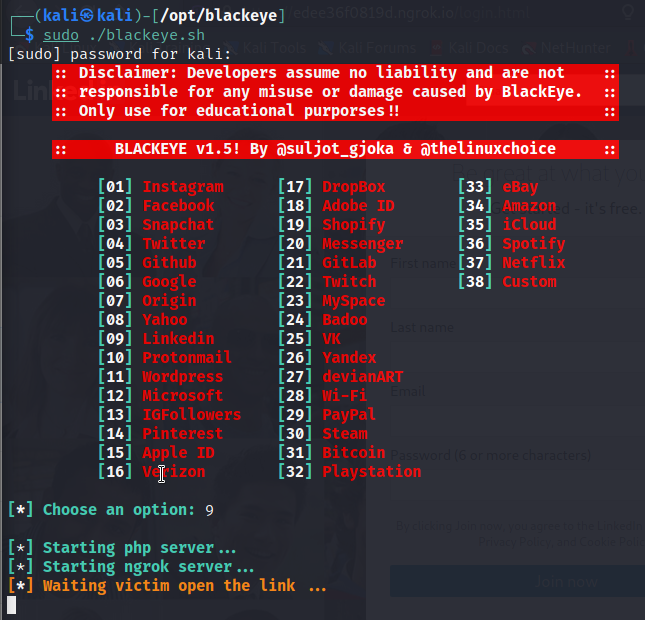
\includegraphics{first.png}
\end{figure}
\\
\\
\\
\\
\\
\\
We chose the option for which phishing site we want to use. 
And then we setup a reverse proxy using a tool named ngrok (https://ngrok.com)
ngrok is a cross-platform application that enables developers to expose a local development server to the Internet with minimal effort. The software makes your locally-hosted web server appear to be hosted on a subdomain of ngrok.com, meaning that no public IP or domain name on the local machine is needed.\\





\begin{figure}[htbp]
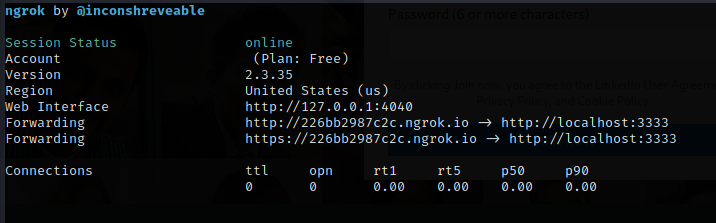
\includegraphics{second.png}
\end{figure}
Then we send this link to the victim.\\
\begin{figure}[htbp]
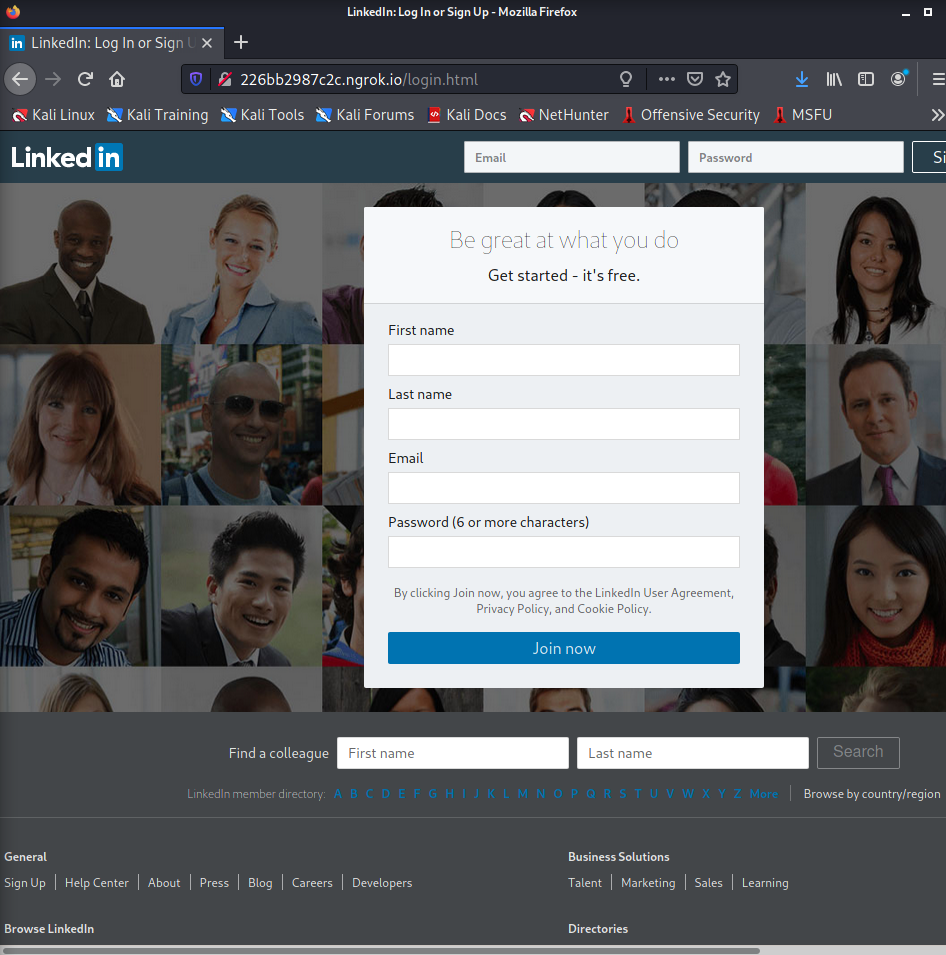
\includegraphics{third.png}
\end{figure}

And then if the victim enters the username and password it is saved in the attackers machine.\\
\\
\\
\\
\\
\\
\\
\\
\\
\\
\\
\\
\\
\\
\\
\\
\\
\\
\\
\\
\\
\\
\\
\\
\\
\\
\\


\begin{figure}[htbp]
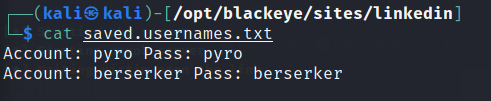
\includegraphics{fourth.png}
\end{figure}\\

And then the link is redirected to the original site and thus the victim can not know about the attack.\\ 





\subsection{SQL Injections}
SQL injection is a web security vulnerability that allows an attacker to interfere with the queries that an application makes to its database. It generally allows an attacker to view data that they are not normally able to retrieve. This might include data belonging to other users, or any other data that the application itself is able to access. In many cases, an attacker can modify or delete this data, causing persistent changes to the application's content or behavior.

In some situations, an attacker can escalate an SQL injection attack to compromise the underlying server or other back-end infrastructure, or perform a denial-of-service attack.

\subsection{XSS attacks}
Cross-site Scripting (XSS) is a client-side code injection attack. The attacker aims to execute malicious scripts in a web browser of the victim by including malicious code in a legitimate web page or web application. The actual attack occurs when the victim visits the web page or web application that executes the malicious code. The web page or web application becomes a vehicle to deliver the malicious script to the user’s browser. Vulnerable vehicles that are commonly used for Cross-site Scripting attacks are forums, message boards, and web pages that allow comments.

A web page or web application is vulnerable to XSS if it uses unsanitized user input in the output that it generates. This user input must then be parsed by the victim’s browser. XSS attacks are possible in VBScript, ActiveX, Flash, and even CSS. However, they are most common in JavaScript, primarily because JavaScript is fundamental to most browsing experiences.

\section{How to Avoid}

Discussing a possible way to avoid attacks:\\
A) Check the source\\\\ 1) dont install from unknown resources\\
2) dont insatll the softwares you dont need\\
3) dont click unknown links\\\\
B)Maintain social information leaks:\\
1) dont use same password for different
websites.It will break the loop if someone
is trying to hack you!\\
2) dONT post about your ongoing projects\\
in the company on social media, as the
attacker may come to know which version
of software you are using and with a known
vulnerablity they can exploit.\\
3) when going out at lunch or break, dont
talk about your works.\\\\
C)Secure your devices:\\
1) importance of antiviruses and firewalls\\
2) Keep system updated!\\
3) Dont root your phone!\\
4) 2FA\\
5) Dont trust anyone!!!\\





\section{Scope of improvement}
Attackers are advancing everyday. New attack vectors are developed everyday, So we can develop ways to defend towards the evergrowing new attack methods. And as Humans are the weakest link in a social engineering attack, then these attacks can never be eliminated. So the defence towards these attacks should be improved.


\begin{thebibliography}{widest entry}
	\bibitem{cite_key1} Breda, F., Barbosa, H. and
Morais, T., 2017, March.
Social engineering and cyber security. In Proceedings
of the International Conference on Technology, Education and Development, Valencia, Spain (pp. 6-8).
	

\end{thebibliography}


\end{document}